\documentclass[a4paper,10pt,english]{article}
\usepackage[utf8]{inputenc}
\usepackage[english]{babel}

\usepackage{amsmath,graphicx,varioref,verbatim,amsfonts,geometry}
\usepackage[usenames,dvipsnames,svgnames,table]{xcolor}
\usepackage[export]{adjustbox}

\usepackage[colorlinks]{hyperref}
\hypersetup{linkcolor=black}

\setlength{\parindent}{0mm}
\setlength{\parskip}{1.5mm}

\usepackage{textcomp}
\definecolor{listinggray}{gray}{0.9}
\definecolor{lbcolor}{rgb}{0.9,0.9,0.9}

\usepackage{listings}
\lstdefinelanguage{python}
{
	morekeywords={print,abs,for,def,if,while,do,break,return,from,import,try,except,else,elif},
	sensitive=false,
	morecomment=[l]{\#}
}
\lstset{language=python,
	backgroundcolor=\color[rgb]{.95,.95,.95},
	numbers=left,xleftmargin=10pt,
	numberstyle=\tiny,stepnumber=1,numbersep=5pt,
	stringstyle=\color{red},
	basicstyle=\footnotesize \ttfamily,
	keywordstyle=\color{blue},
	commentstyle=\color{green},
	basewidth=0.60em,
	showstringspaces=false,
	captionpos=b,
	frame=single
}

\renewcommand{\thesubsection}{\alph{subsection}.}
\renewcommand{\thesubsubsection}{\normalfont\roman{subsubsection}.}

\begin{document}

\begin{titlepage}
    \begin{center}
        \vspace*{1cm}
            
        \Huge
        \textbf{Molecular Dynamics Project}
            
        \vspace{0.5cm}
        \LARGE
        FYS-MEK1110
            
        \vspace{1.5cm}
            
        \textbf{William Dugan}
            
        \vfill
    
        \begin{figure}[h!] 
            \centering 
            
\includegraphics[scale=.7]{../figures/uio_logo.pdf} 
        \end{figure}    
        
        \Large
        University of Oslo\\
        March, 2022
    \end{center}
\end{titlepage}

\newpage
{
  \tableofcontents
}

\newpage

\section{Introduction} \label{1}

The goal of this project is to model an argon gas, where the atoms interact according to the famous Lennard-Jones potential,
\begin{align} \label{eq:1}
    U(r) = 4 \epsilon 
    \left(
        \left( 
            \frac{\sigma}{r}
        \right)^{12} 
        - \left(
            \frac{\sigma}{r}
        \right)^6
    \right)
\end{align}
where $r$ is the distance between two atoms, $r=||\Vec{r_i}-\Vec{r_j}||$. The parameters $\sigma$ and $\epsilon$ determine which chemical compound is modelled.

The full code used to answer the tasks will not be shown in this document. See \url{https://github.com/willidu/FYS-MEK1110/tree/main/md-prosjekt}.

I am greatfull for the advice recieved from our advisor as well as my fellow students undertaking this project. It would not be possible to finish the project without their help. 

\subsection{Understanding the potential} \label{1a}

\begin{figure}[h!]
    \centering 
    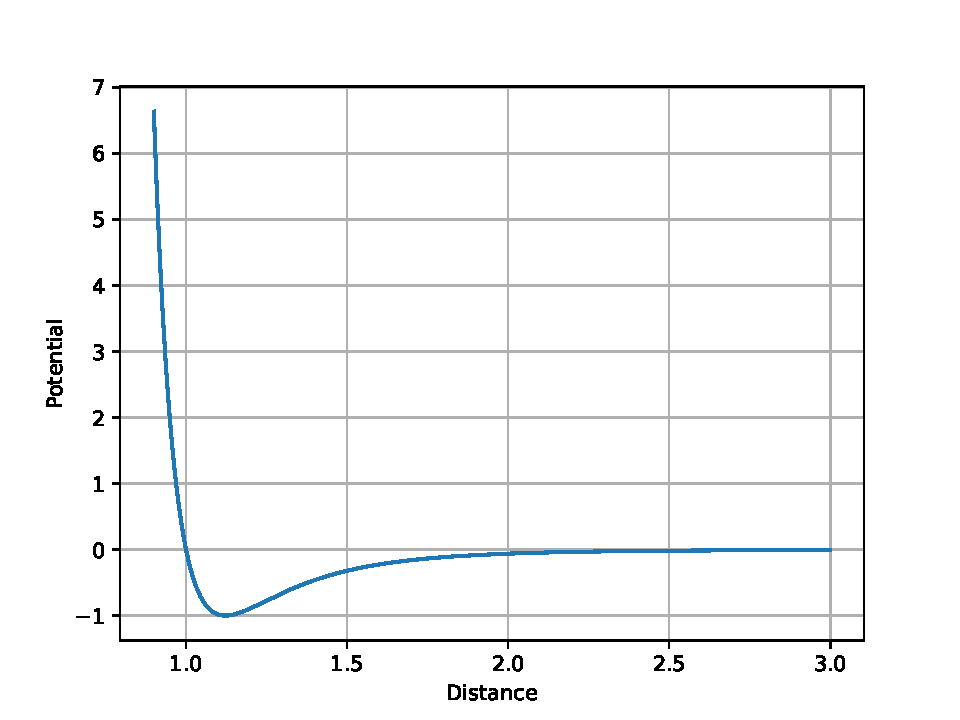
\includegraphics[scale=.65]{../figures/1_a_i.pdf} 
    \caption{Plot of $U(r)$ for $r\in[0.9, 3], \epsilon=1, \sigma=1$.}
    \label{fig:plot1}
\end{figure}

The behaviour of $U(r)$ is vastly different for $r<\sigma$ and $r>\sigma$. For $r<\sigma$, the first term in equation \ref{eq:1} dominates and will make the potential go towards $\infty$ for small $r$. For $r=\sigma$ the terms are equal and the potential is 0. For $r>\sigma$, the second term in equation \ref{eq:1} dominates hence the negative potential. For $r\to \infty$ the potential will be 0 again. The two terms quickly becomes the same order of magnitude, effectively giving us a 0 potential a lot earlier than $r=\infty$.

\newpage
The equilibrium is reached when the force between the two atoms is zero. The force is given by
\begin{align}
    \Vec{F}(\Vec{r}) = - \nabla U(\Vec{r})
\end{align}
Since we are only considering one dimension (for now), this will be
\begin{align}
    F(r) &= - \frac{dU}{dr} \\
    &= -(-4*12\epsilon\sigma^{12}r^{-13} + 4*6\epsilon\sigma^{6}r^{-7}) \\
    &= -\frac{24\epsilon\sigma^{12}(r^6-2\sigma^6)}{r^{13}} \label{eq:5}
\end{align}
If we solve equation \ref{eq:5} equal to zero, we get our points of equilibrium. We get the following solutions:
\begin{align*}
    r 
    = \sqrt[\leftroot{-2}\uproot{2}6]{2\sigma^6} 
    = \sigma \sqrt[\leftroot{-2}\uproot{2}6]{2} 
    \hspace{1cm} \land \hspace{1cm}
    r
    =\infty
\end{align*}

Since the potential is at a minimum at $ r = \sigma \sqrt[6]{2} $, this is a stable equilibrium point. Contrary to this, $ r = \infty $ is an unstable equilibrium since the potential is at a (local) maximum.

The motion of two atoms starting with a separation of $1.5\sigma$ can be described by the graph of the potential (Figure \ref{fig:plot1}). At $r=1.5\sigma$ the slope of $U$ is positive, so the force between the atoms will be in negative $r$ direction. This means that the atom will move towards the left until it reaches the potential $U(1.5\sigma)$ at the graph to the left of the equilibrium point.  Since energy is conserved in this case, atom will simply oscillate between these points.

If the atoms had an initial separation of $0.95\sigma$, the force would initially be in the positive $r$ direction. The atom would then move in this direction forever, since it cannot reach the potential $U(0.95\sigma)$ on the right side of the equilibrium point.

\subsection{Forces and equation of motion} \label{1b}

The (vector)force on atom $i$ at position $\Vec{r_i}$ from atom $j$ at position $\Vec{r_j}$ follows from equation \ref{eq:5} and is given by
\begin{align} \label{eq:6}
    \Vec{F}
    = - \frac{24\epsilon\sigma^{12}(r^6-2\sigma^6)}{r^{13}} \frac{\Vec{r}}{|\Vec{r}|}
\end{align} 
where 
\begin{align*}
    \frac{\Vec{r}}{|\Vec{r}|} = \frac{\Vec{r_i} - \Vec{r_j}}{||\Vec{r_i} - \Vec{r_j}||}
\end{align*}
is the unit vector in the direction of the force. 

To find the equation of motion for atom $i$ we can use Newton's second law and equation \ref{eq:6}.
\begin{align} \label{eq:12}
    \sum \Vec{F} &= m\Vec{a} \\
    \implies\Vec{a_i} &= \frac{d^2\Vec{r_i}}{dt^2} = \frac{\sum \Vec{F_i}}{m} \\
    &= \frac{1}{m} \sum_{j\neq i}{\left [-\frac{24\epsilon\sigma^6(r^6-2\sigma^6)}{r^{13}}\right] \frac{\Vec{r_i} - \Vec{r_j}}{||\Vec{r_i} - \Vec{r_j}||}} \\
    &= \frac{24\epsilon}{m} \sum_{j\neq i}{\left[-\frac{\sigma^6}{r^{11}} + \frac{2\sigma^{12}}{r^{13}}\right] \frac{\Vec{r_i} - \Vec{r_j}}{||\Vec{r_i} - \Vec{r_j}||}} \\
    &= \frac{24\epsilon}{m} \sum_{j\neq i}{\left[{2\left( \frac{\sigma}{r}\right)^{12} - \left( \frac{\sigma}{r}\right)^{6}}\right] \frac{1}{r} \frac{\Vec{r_i} - \Vec{r_j}}{||\Vec{r_i} - \Vec{r_j}||}} \\
    &= \frac{24\epsilon}{m} \sum_{j\neq i}{\left[{2\left( \frac{\sigma}{||\Vec{r_i} - \Vec{r_j}||}\right)^{12} - \left( \frac{\sigma}{||\Vec{r_i} - \Vec{r_j}||}\right)^{6}}\right] \frac{\Vec{r_i} - \Vec{r_j}}{{||\Vec{r_i} - \Vec{r_j}||}^2}}
\end{align}
We sum for all $j \neq i$ since an atom $i$ will interact with all other atoms except itself.

\subsection{Units} \label{1c}

To write equation \ref{eq:12} in dimensionless form, we use $\Vec{r_i}^*=\Vec{r_i}/\sigma$ and $t^*=t/\tau$. We also have to assume $\sigma>0$.
\begin{align}
    \frac{d^2 \Vec{r_i}^*}{d{t^*}^2} 
    &= 24 \sum_{j\neq i}{\left[{2\left( \frac{\sigma}{||\Vec{r_i}^*\sigma - \Vec{r_j}^*\sigma||}\right)^{12} - \left( \frac{\sigma}{||\Vec{r_i}^*\sigma - \Vec{r_j}^*\sigma||}\right)^{6}}\right] \frac{\Vec{r_i}^*\sigma - \Vec{r_j}^*\sigma}{{||\Vec{r_i}^*\sigma - \Vec{r_j}^*\sigma||}^2}} \\
    &= 24 \sum_{j\neq i}{\left[{2\left( \frac{\sigma}{|\sigma|*||\Vec{r_i}^* - \Vec{r_j}^*||}\right)^{12} - \left( \frac{\sigma}{|\sigma|*||\Vec{r_i}^* - \Vec{r_j}^*||}\right)^{6}}\right] \frac{\Vec{r_i}^* - \Vec{r_j}^*}{{||\Vec{r_i}^* - \Vec{r_j}^*||}^2}} \\
    &= 24 \sum_{j\neq i}{\left[{2{||\Vec{r_i}^* - \Vec{r_j}^*||}^{-12} - {||\Vec{r_i}^* - \Vec{r_j}^*||}^{-6}}\right] \frac{\Vec{r_i}^* - \Vec{r_j}^*}{{||\Vec{r_i}^* - \Vec{r_j}^*||}^2}} 
\end{align}

To find the characteristic time scale $\tau$, we perform a simple dimension analysis and compare the units of $\tau$ and the constants given.
\begin{align*}
    \sigma &= [m] \\
    m &= [kg] \\
    \epsilon &= [J] = \left[ \frac{kg \cdot m^2}{s^2} \right]
\end{align*}
Since we need $\tau$ to be dimensionless, it has to be the same unit as $t$, hence seconds. Therefore, $\tau$ is given by
\begin{align*}
    \tau = \sqrt{\frac{kg \cdot m^2}{kg \cdot m^2} \cdot s^2} = [s]
\end{align*}
which is achieved by expressing $\tau$ the following way:
\begin{align}
    \tau = \sqrt{\frac{m\sigma^2}{\epsilon}}
\end{align}
The values for argon are 
\begin{align*}
    \sigma &= 3.405 \cdot 10^{-10} \text{m}, \\
    m &= 39.95 \cdot 1.66 \cdot 10^{-27} \text{kg}, \\
    \epsilon &= 1.0318 \cdot 1.602 \cdot 10^{-21} \text{J}
\end{align*}
which gives $\tau \approx 2.26 \cdot 10^{-12}$s.

\newpage

\section{Two-atom simulations} \label{2}

See \verb|md-prosjekt/task2.py|.

\subsection{Implementation} \label{2a}

See \verb|md-prosjekt/two_atom_sim.py|. Even though the task asked for only one function, I chose to separate it into multiple functions. This made it easier to debug.

\subsection{Motion} \label{2b}

\begin{figure}[h!] 
    \centering 
    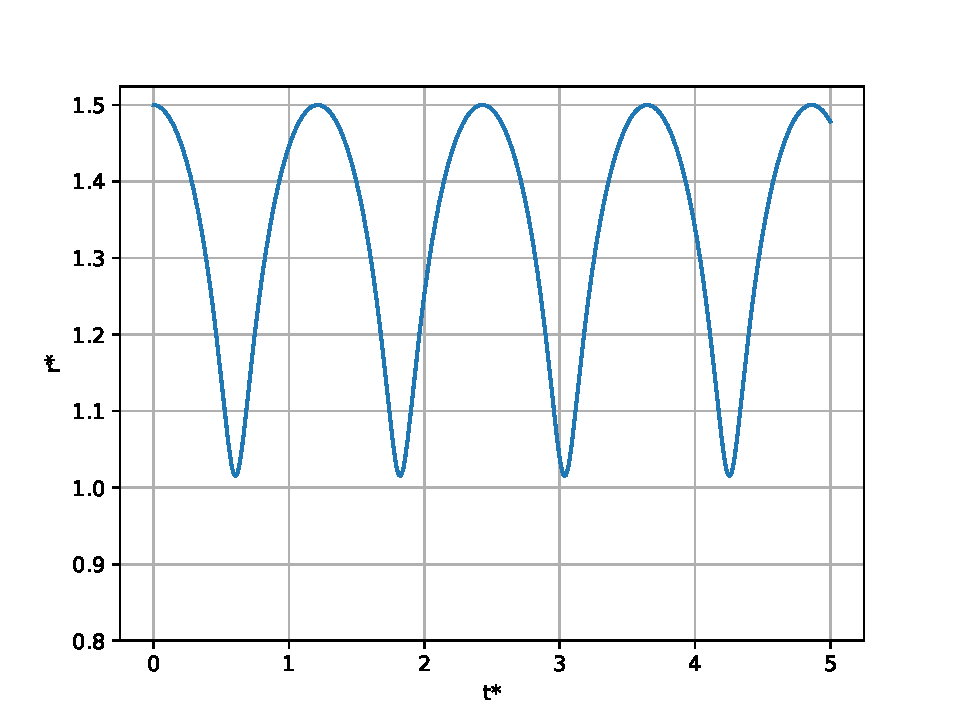
\includegraphics[scale=.65]{../figures/2_b_ii.pdf} 
    \caption{Plot of $r^*$ for $t^*\in[0, 5]$. Initial separation 1.5$\sigma$.}
    \label{fig:plot2}
\end{figure}

As we found in \textit{\nameref{1b}}, the expected motion of two atoms with an initial separation of $1.5\sigma$ is periodic. From Figure \ref{fig:plot2} we see that the atoms oscillate periodically between two points. This tells us that our model works as expected.

We will now simulate with an initial separation of $.95\sigma$. See figure \ref{fig:plot3}. Here we can see that the atoms move away from each other. They do this with a constant velocity, as the acceleration goes to zero (equation \ref{eq:5}). We also notice that the curve straightens out very quickly, which is explained by Figure \ref{fig:plot1} when the potential goes towards infinity for small $r$. This motion is also as expected. 

\begin{figure}[h!]
    \centering 
    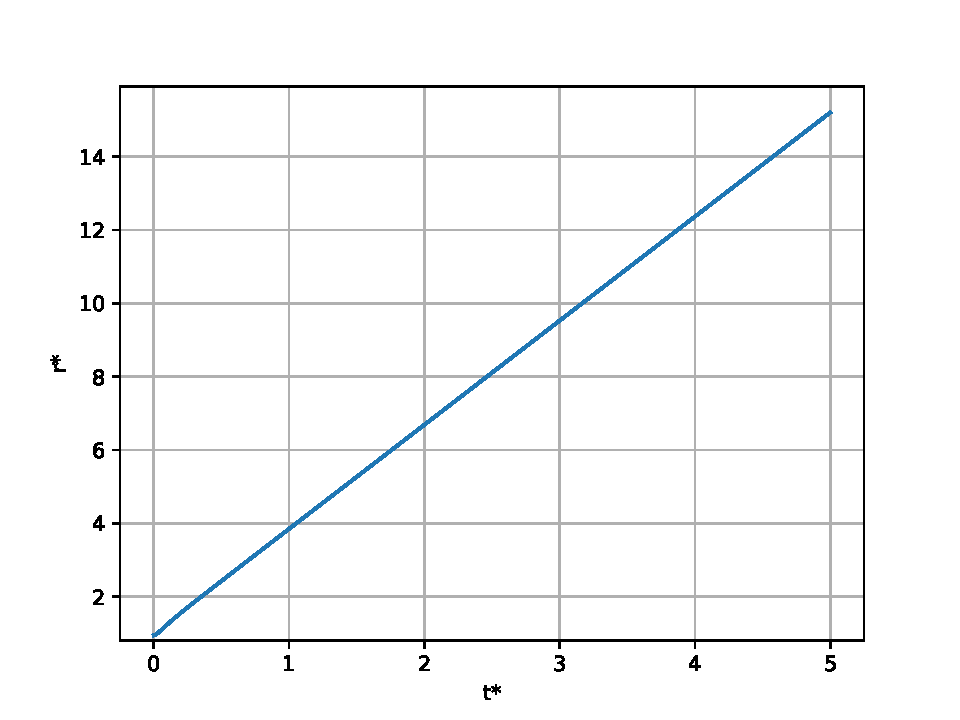
\includegraphics[scale=.65]{../figures/2_b_iv.pdf} 
    \caption{Plot of $r^*$ for $t^*\in[0, 5]$. Initial separation .95$\sigma$.}
    \label{fig:plot3}
\end{figure}

\newpage

\subsection{Energy} \label{2c}

In order to do anything regarding potential energy, we have to find an expression for the potential energy in dimensionless form. Remembering that $r^*$ is already scaled by $\sigma$, $\Vec{r_i}^* = \Vec{r_i} / \sigma$, we get the following equation by dividing equation \ref{eq:1} with $\epsilon$. This leaves
\begin{align}
    U^*(r^*) = 4 
    \left(
        {r^*}^{-12} - {r^*}^{-6} 
    \right)
\end{align}
where $r^*=||\Vec{r_i}^* - \Vec{r_j}^*||$.

\begin{figure}[h]
    \centering
    \begin{minipage}{0.5\textwidth}
        \centering
        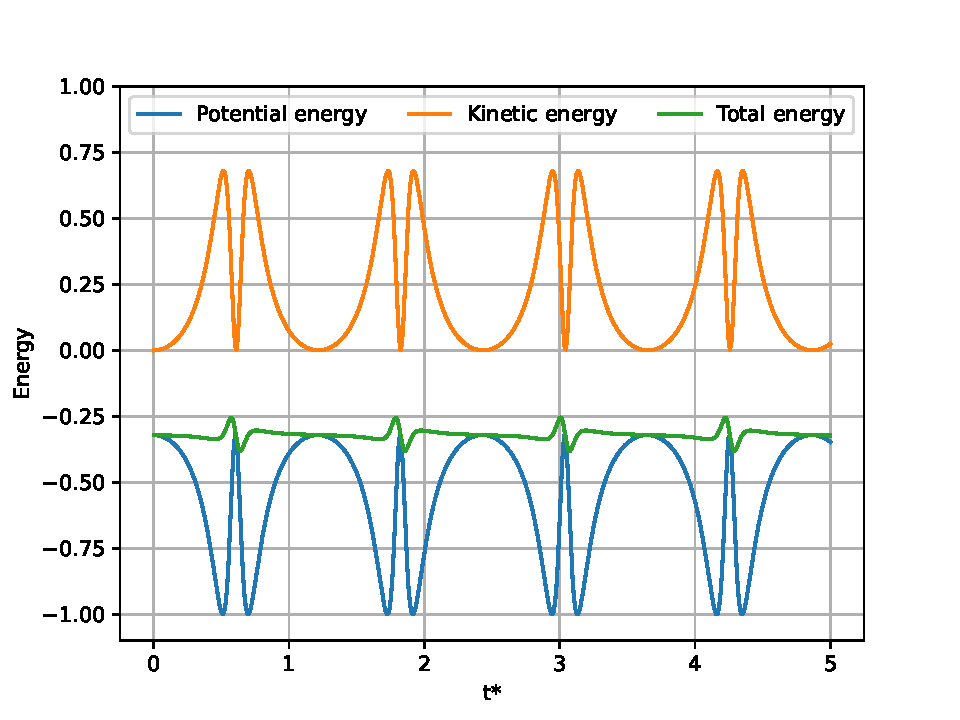
\includegraphics[width=1.05\textwidth]{../figures/2_c_i_1.pdf}
    \end{minipage}\hfill
    \begin{minipage}{0.5\textwidth}
        \centering
        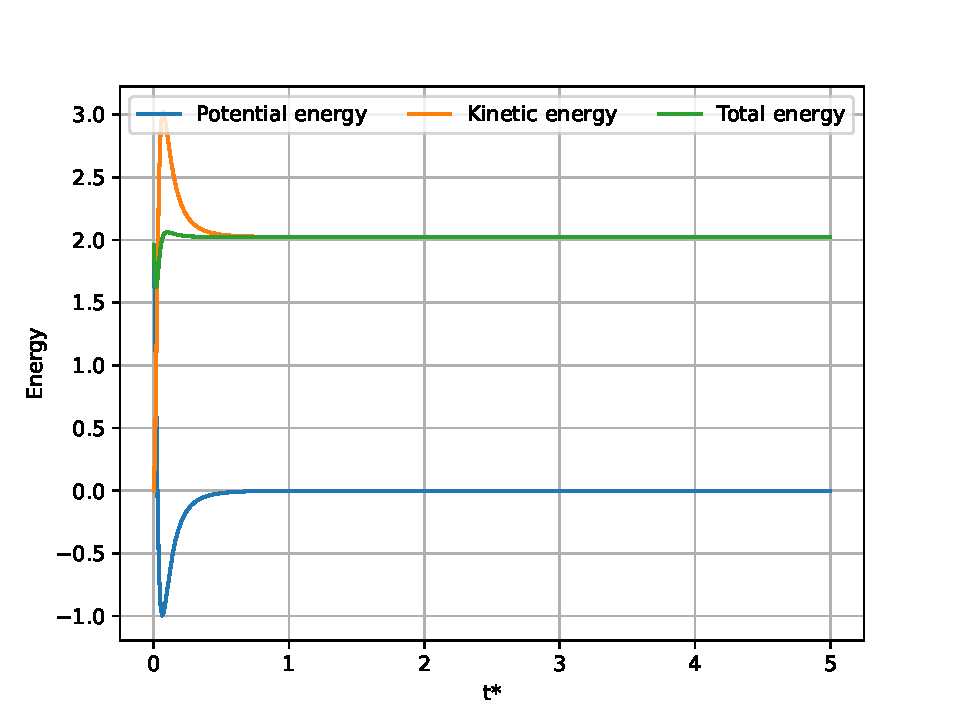
\includegraphics[width=1.05\textwidth]{../figures/2_c_i_2.pdf}
    \end{minipage}
    \caption{Energy plot with separation $1.5\sigma$ and $.95\sigma$ for $t\in[0, 5]$.}
    \label{fig:energyplots1}
\end{figure}

\newpage

In theory, the total energy should be conserved since we do not have any non-conservative forces. If we compare the total energy for the two simulations, we get results consistent with the findings in \textit{\nameref{1b}}. If energy had been lost, the particles would slow down and the time period for each oscillation would increase. This is not the case. Hence, energy is conserved. We see from Figure \ref{fig:energyplots1} that momentum is conserved if the initial separation is $1.5 \sigma$, but it is not conserved when it is $0.95 \sigma$.

\begin{figure}[h]
    \centering
    \begin{minipage}{0.5\textwidth}
        \centering
        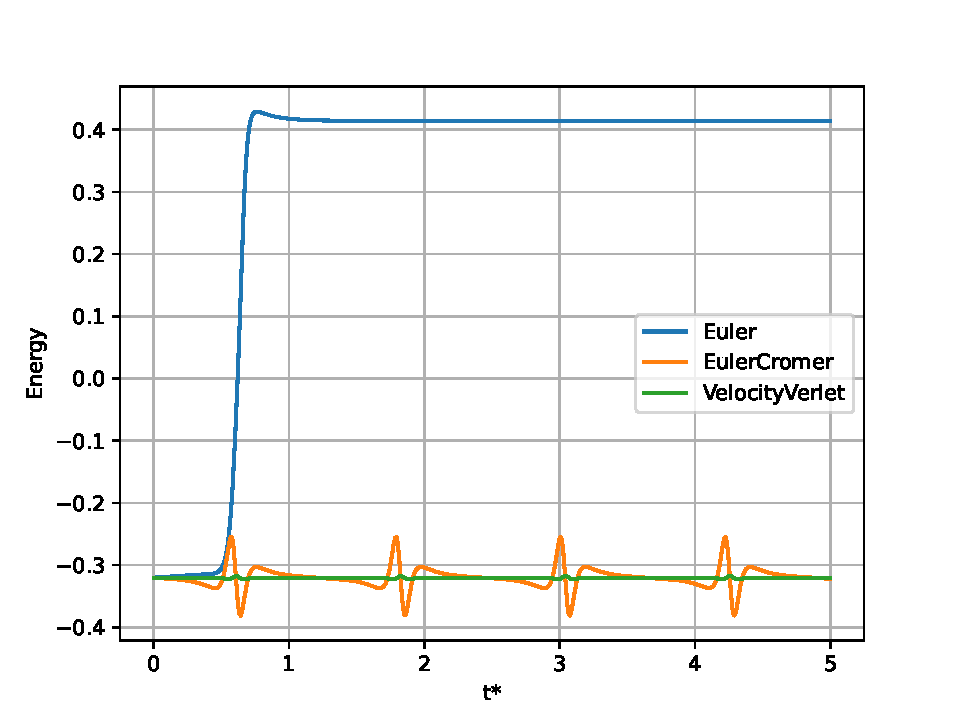
\includegraphics[width=1.05\textwidth]{../figures/2_c_iv_15.pdf}
    \end{minipage}\hfill
    \begin{minipage}{0.5\textwidth}
        \centering
        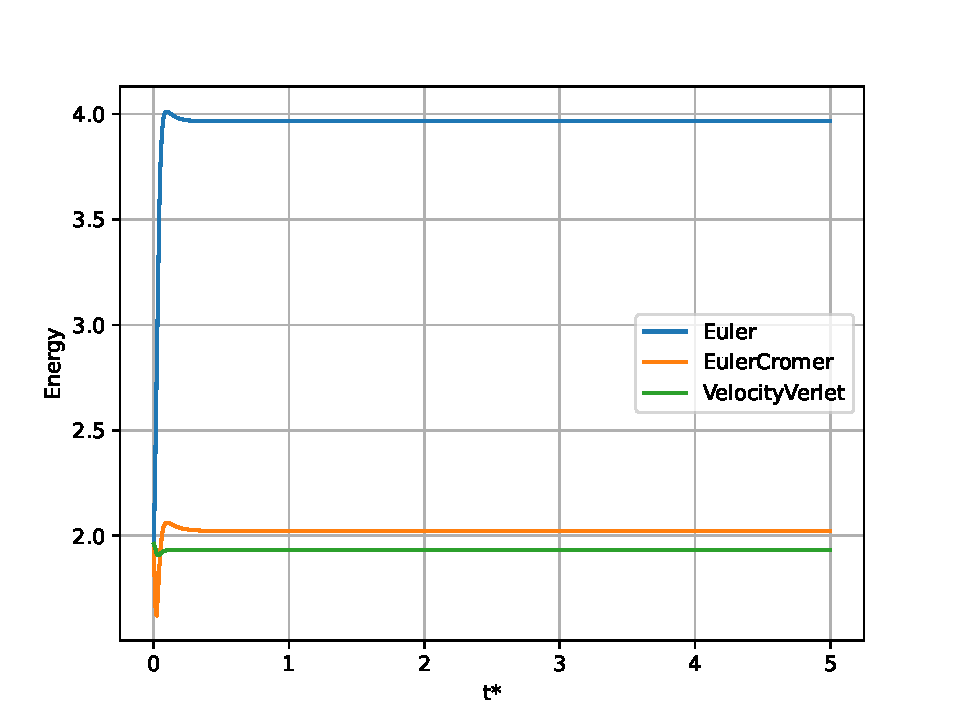
\includegraphics[width=1.05\textwidth]{../figures/2_c_iv_095.pdf}
    \end{minipage}
    \caption{Total energy with initial separation $1.5\sigma$ for $t\in[0, 5]$ and $.95\sigma$ and $t\in[0, 1]$ respectively.}
    \label{fig:energyplots2}
\end{figure}

From Figure \ref{fig:energyplots2} it is clear that energy is not conserved with the Euler method. Let us consider the situation with an initial separation of $1.5\sigma$. It is clear that even though there are some fluctuations with both the Euler-Cromer and Velocity Verlet methods, the changes are periodic and does not increase with time. This is not the case for the Euler method. we can observe the same occurrence then the initial separation is $.95\sigma$. One last observation is that the total energy is one order of magnitude larger when the initial separation is $.95\sigma$ when compared to the total energy for $1.5\sigma$.

I was unable to get a stable motion with Euler's method, even with unreasonably small time steps. Using $\Delta t = 0.01$ I got stable motion and conservation of energy with Euler-Cromer and Velocity Verlet. It is well known that Euler-Cromer is far better than Euler when working with periodic movement. The differences between these two methods are minor, and it is not more difficult in any way to use Euler-Cromer. Velocity Verlet is a more intuitive integration method as it is based on Taylor approximations of the equations for motion. We will use this method for the rest of the project.

\newpage

\subsection{Visualization} \label{2d}

\begin{figure} [h!]
    \centering
    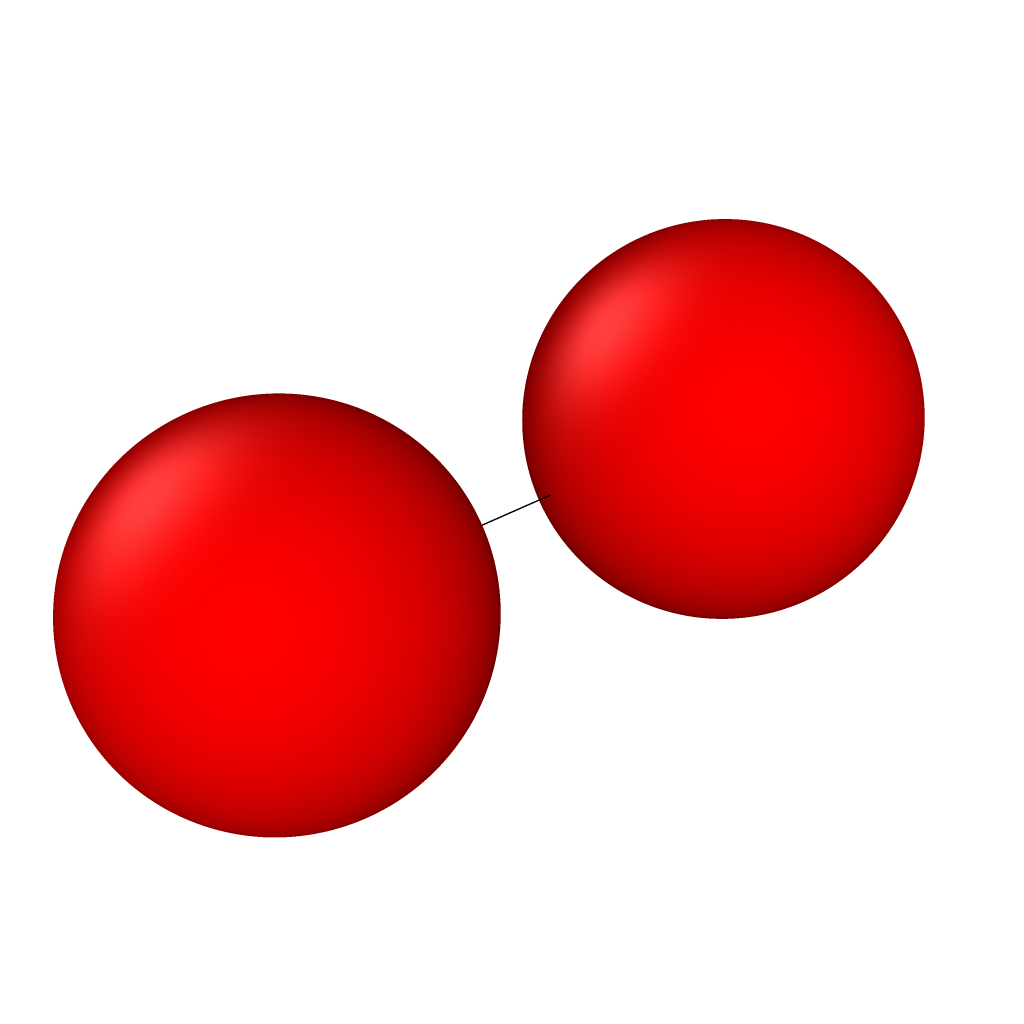
\includegraphics[scale=0.25]{../figures/2_d_ii_1.png}
    \caption{Representation of .xyz file in Ovito, showing one frame only.}
    \label{fig:ovito1}
\end{figure}

\newpage

\section{Large systems} \label{3}

See \verb|md-prosjekt/task3.py|.

\subsection{Implementation} \label{3a}
See \verb|md-prosjekt/n_atom_sim.py|. Note that the code does not use Newton's third law to reduce the number of force calculations. To reduce the simulation time we set a cutoff in the potential $r_c^*$; we see from Figure \ref{fig:plot1} that the potential is effectively zero at $r=3$, which is the value we chose for our cutoff.

\begin{figure} [h!]
    \centering
    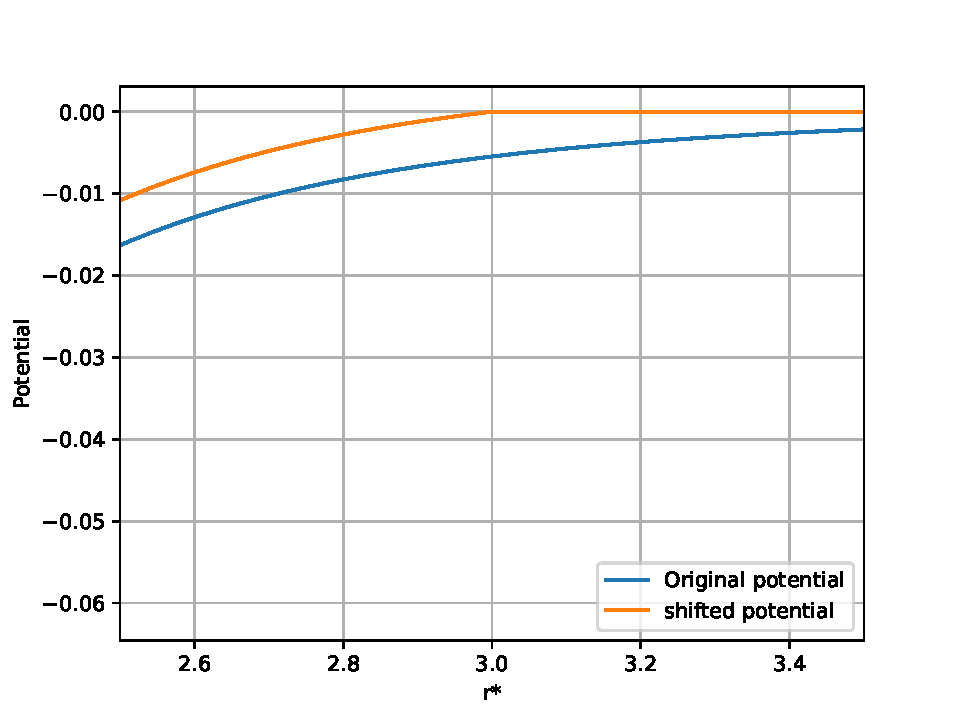
\includegraphics[scale=0.65]{../figures/3_a_iv.pdf}
    \caption{Plot of original and shiftet potential for $r^* \in [2.5, 3,5]$ with $r_c^* = 3$.}
    \label{fig:shiftedpotential}
\end{figure}

We obserce that the potential if shifted with $U^*(3)$ for $r^*<3$. This does not affect force calculations as it is defined by the derivative of the potential, so the addition of a constant does not have any effect.

\newpage

\subsection{Verification} \label{3b}

The solver for N atoms also works for two atoms, and yields the same results as \textit{\nameref{2}}. We will now simulate the motion of four atoms. The first simulation is run with initial positions [1, 0, 0], [0, 1, 0], [-1, 0, 0] and [0, -1, 0]. For the second simulation, we alter the first atom to have a starting position of [1, 0.1, 0].

\begin{figure}[h]
    \centering
    \begin{minipage}{0.5\textwidth}
        \centering
        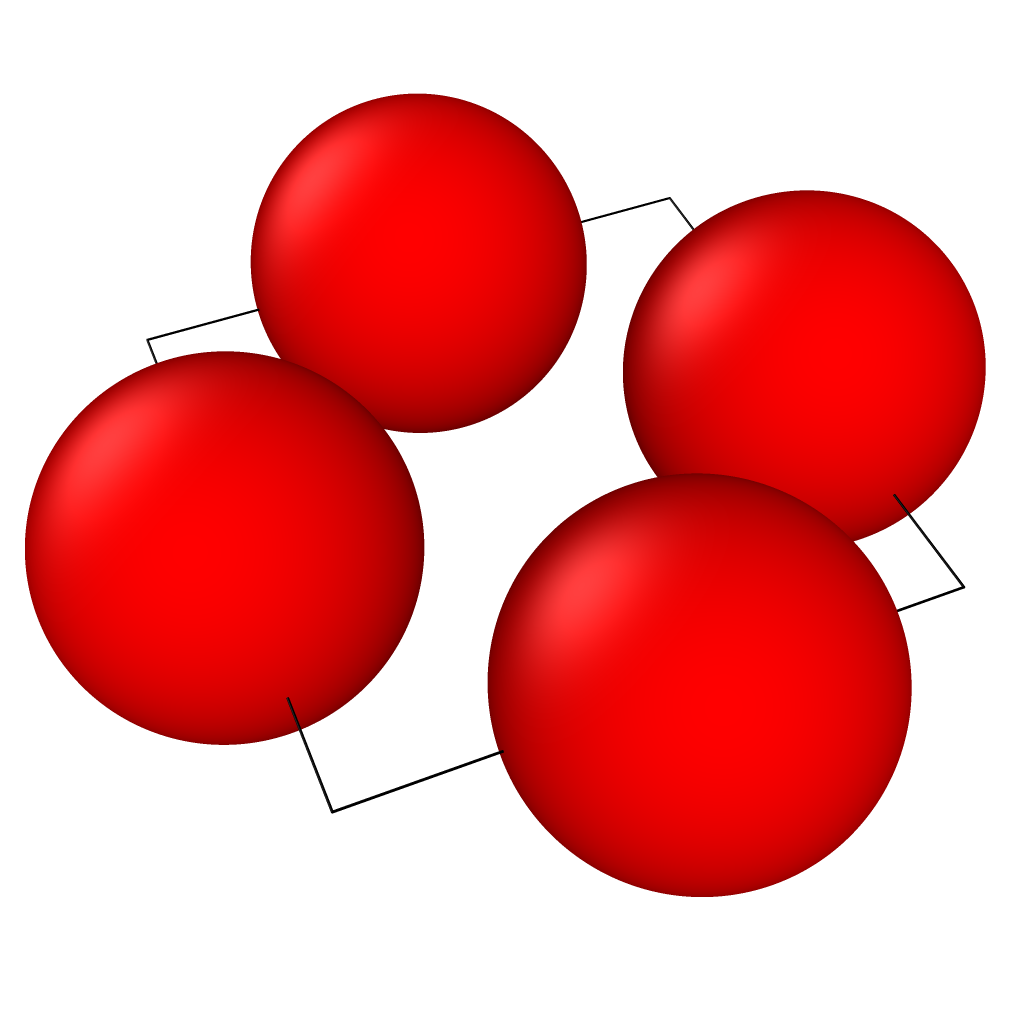
\includegraphics[width=0.65\textwidth]{../figures/3_b_iii_1.png}
    \end{minipage}\hfill
    \begin{minipage}{0.5\textwidth}
        \centering
        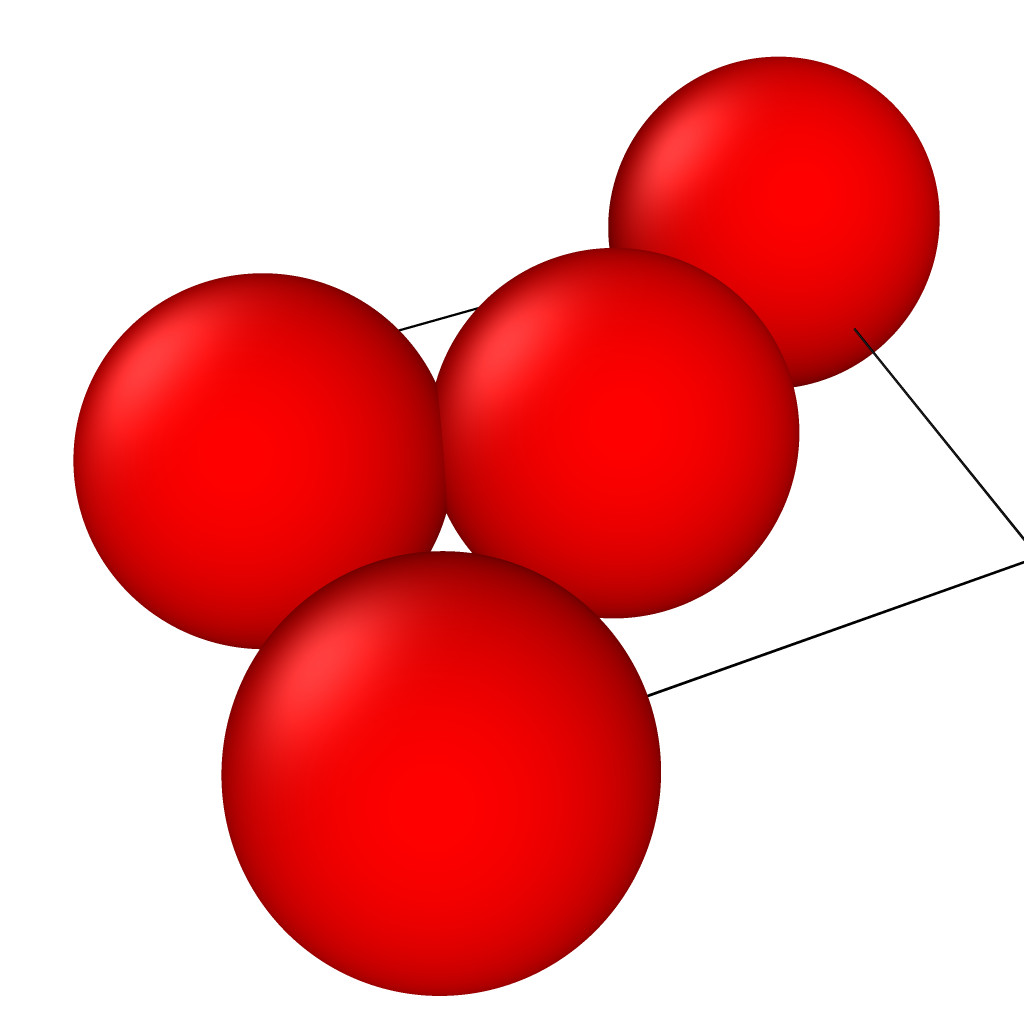
\includegraphics[width=0.65\textwidth]{../figures/3_b_iii_2.png}
    \end{minipage}
    \caption{Ovito visualization for the last simulation, showing frame 1/500 and 415/500.}
    \label{fig:ovito2}
\end{figure}

\begin{figure}[h]
    \centering
    \begin{minipage}{0.5\textwidth}
        \centering
        
\includegraphics[width=1.05\textwidth]{../figures/3_b_iv.pdf}
    \end{minipage}\hfill
    \begin{minipage}{0.5\textwidth}
        \centering
        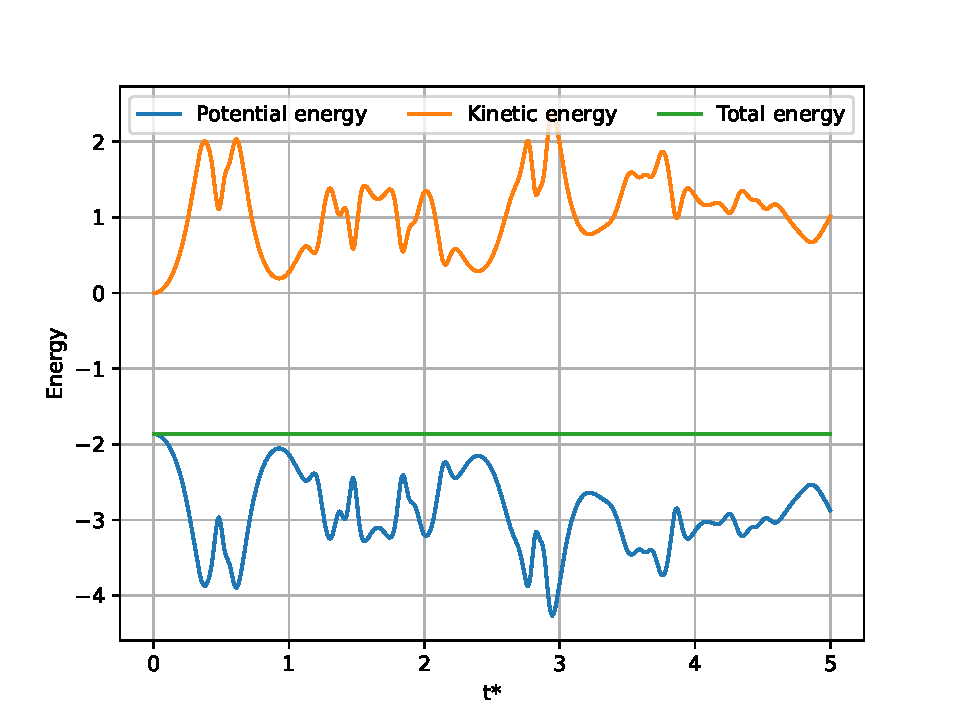
\includegraphics[width=1.05\textwidth]{../figures/3_b_v.pdf}
    \end{minipage}
    \caption{Energy plot for simulations with four atoms starting from rest.}
    \label{fig:energyplots3}
\end{figure}

We observe that we get a neat periodic movement for the atoms if the system is symtric, which is reasonable as the forces on the atoms are only of different direction but has the same magnitude. We also observe that the energy is conserved in both simulations.

\newpage

\subsection{Initialisation} \label{3c}

See \verb|md-prosjekt/box.py|. Running the script with $n=3$ and $d=20/3$ we get $4*3^3=108$ atoms. See \verb|md-prosjekt/xyz_files/3_c.xyz|. 

\begin{figure}[h!]
    \centering
    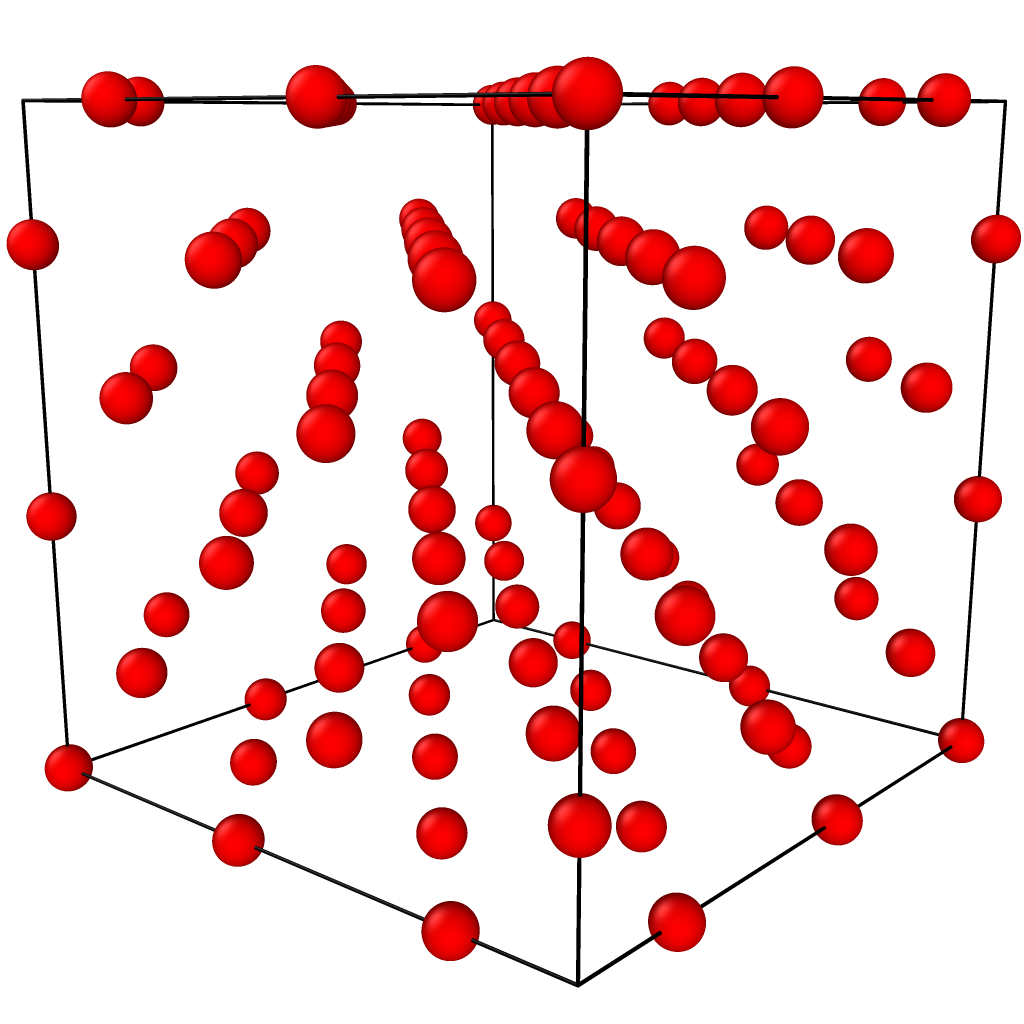
\includegraphics[scale=0.45]{../figures/3_c.png}
    \caption{Ovito visualisation of the face-centered lattic structure with 108 atoms.}
    \label{fig:ovito3}
\end{figure}

To show that the unit cell size corresponding to the density $\rho=1.374$ g/cm$^3$ is $d=1.7 \sigma$, we use the general formula for density, $\rho = $total mass/total volume.
\begin{align*}
    \rho
    &= \frac{n \cdot m}{L^3} \\
    &= \frac{4 \cdot 39.95 \cdot 1.66 \cdot 10^{-27} \cdot 10^{3} \text{g}}{{(1.7 \cdot 3.405 \cdot 10^{-10} \cdot 10^2 \text{cm})}^3} \\
    &\approx 1.3676 \left[ \frac{\text{g}}{\text{cm}^3} \right]
\end{align*}
where we have used that $n = 4$, $m = 39.95$ u, $L=1.7\sigma$.

\newpage

\subsection{Many atoms, open boundary} \label{3d}

\begin{figure}[h!]
    \centering
    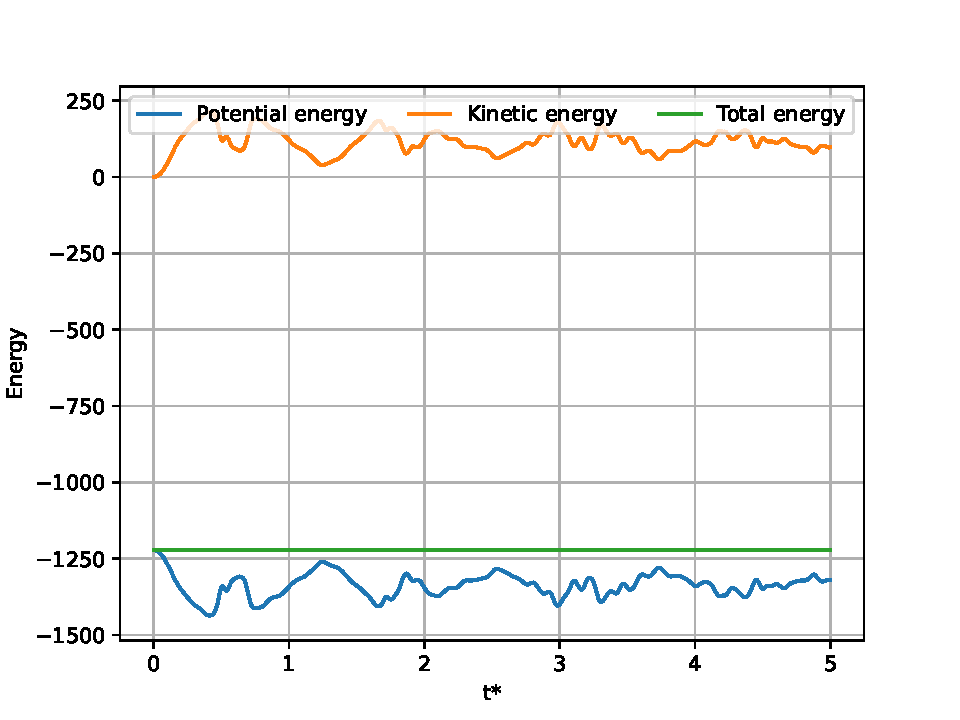
\includegraphics[scale=0.65]{../figures/3_d.pdf}
    \caption{Energy plot for simulation with 256 atoms starting from rest.}
    \label{fig:energyplots4}
\end{figure}

The differences between the simulation with 256 atoms and the non-symetrical simulation with four atoms are minor. We observe the same type of motion but simply with more atoms. Energy is also conserved in this case. Also note that the changes in potential and kinetic energy is initially larger, but decreases quickly as the system reaches equilibrium.

\subsection{Boundary conditions} \label{3e}

I chose to only implement periodic boundary conditions. In order to calculate the shortest distance between two atoms when placing identical systems on all sides of the bounding box, I added the following to the function that calculates the distance between atoms:
\begin{lstlisting}
if self.bound:
    r -= np.around(r/self.L)*self.L
\end{lstlisting}

To move the atoms through the walls I added the following line to my integration loop:
\begin{lstlisting}
if self.bound:
    x_ = np.floor(x[i+1]/self.L)*self.L
    x[i+1] -= x_
    self.wallcount[i+1] = self.wallcount[i] + x_
\end{lstlisting}
The wallcount variable will be used later in the project to calculate mean square displacement and is an array with zeros as default.

\newpage

To test the boundary conditions, we simulate a single atom starting at [1, 0, 0] with velocity \newline [1, 0, 0]. The length of the bounding box is set to 2.

\begin{figure}[h!]
    \centering
    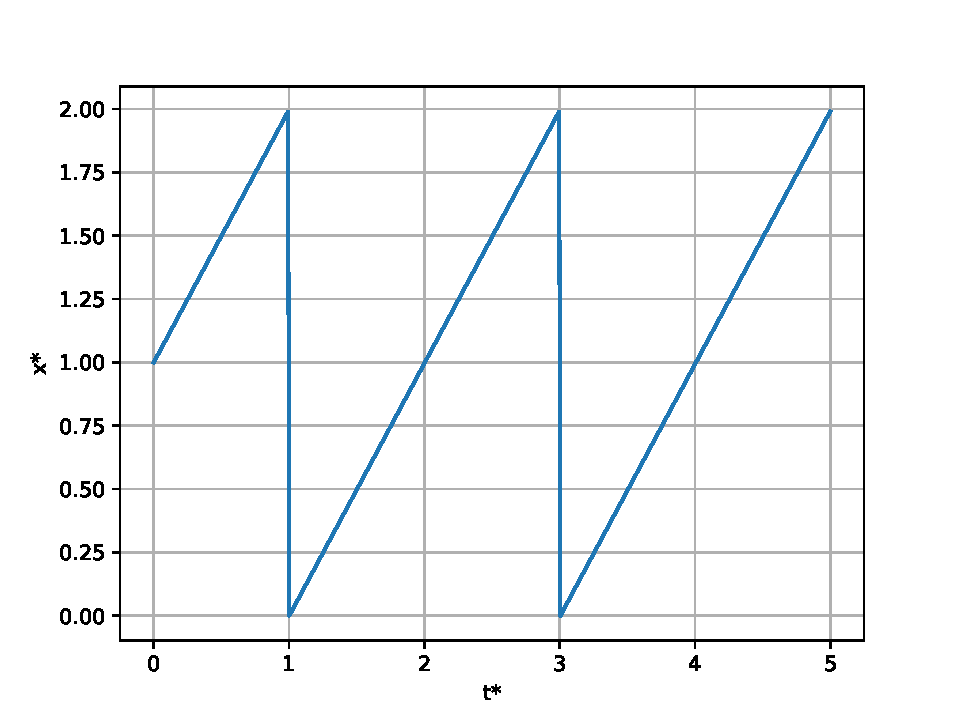
\includegraphics[scale=0.65]{../figures/3_e.pdf}
    \caption{Plot of x-coordinate of atom with periodic boundaries.}
    \label{fig:boundaries}
\end{figure}

The motion is as expected, and our Implementation of periodic boundaries works.

\newpage

\section{Science} \label{4}

See \verb|md-prosjekt/task4.py|. All the simulations are run with $\Delta t = 0.01, d=1.7$ and periodic boundary conditions.

\subsection{Temperature} \label{4a}

\begin{figure}[h!]
    \centering
    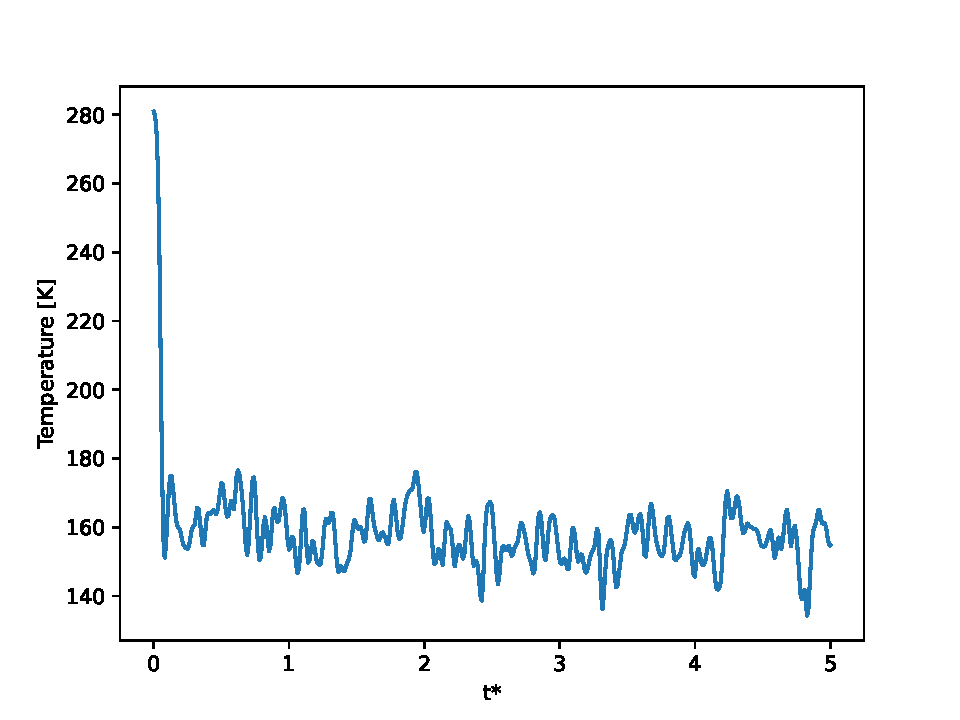
\includegraphics[scale=0.65]{../figures/4_a_ii.pdf}
    \caption{Plot of temperature for 108 atoms with initial temperature of 300K.}
    \label{fig:temperature1}
\end{figure}

To find an initial temperature that yielded equilibrium temperature around 95K I ran 10 simulations with 108 atoms for 5 $t^*$ and averaged the temperature for the last 4.5 $t^*$. By trial and error I found that an initial temperature of 180K gave me an equilibrium temperature around 95K. The rest of the simulations are run with this initial temperature.

\subsection{Velocity autocorrelation and diffusion coefficient} \label{4b}

I am too happy with my one-liner to not include it here:
\begin{lstlisting}[breaklines=true]
def vac(self) -> np.ndarray:
    return np.sum(np.einsum('ijk,jk->ij', self.v, self.v0)/np.einsum('ij,ij->i',self.v0, self.v0), axis=1)/self.n
\end{lstlisting}

\begin{figure}[h]
    \centering
    \begin{minipage}{0.5\textwidth}
        \centering
        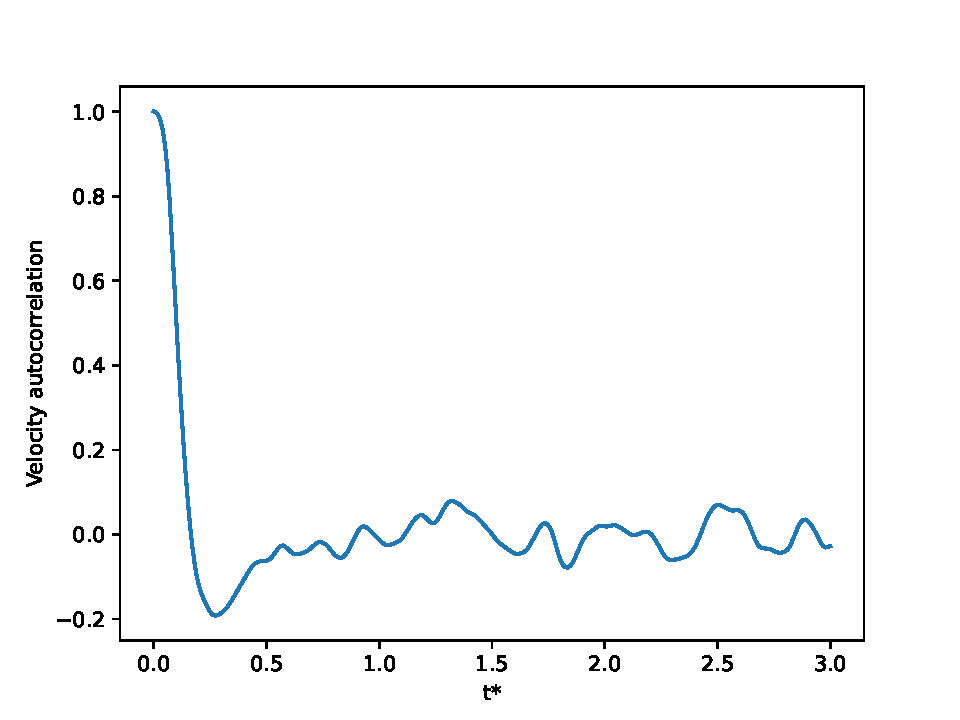
\includegraphics[scale=0.5]{../figures/4_b_ii.pdf}
    \end{minipage}\hfill
    \begin{minipage}{0.5\textwidth}
        \centering
        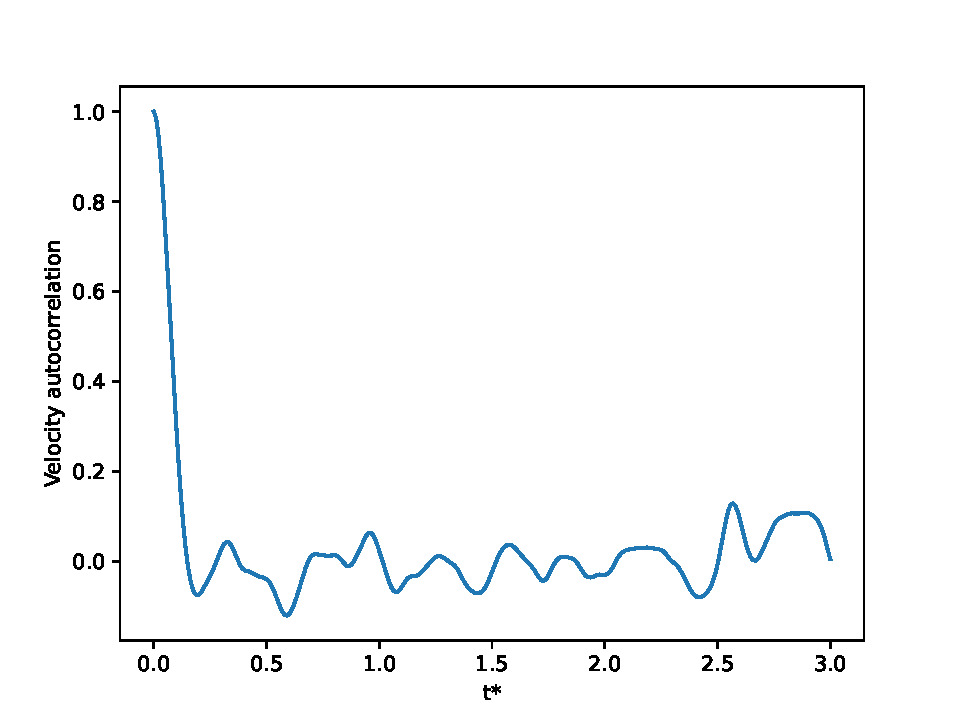
\includegraphics[scale=0.5]{../figures/4_b_iii.pdf}
    \end{minipage}
    \caption{Velocity autocorrelation for 256 atoms. Leftmost is simulated with lattice structure and from rest, rightmost is initially at equilibrium.}
    \label{fig:vac}
\end{figure}

The velocity autocorrelation plotted in figure \ref{fig:vac} is similar to that of A. Rahman and looks to be stabilize around 0 as it should. We observe minor changes in calculating autocorrelation from equilibrium, but the curve does indeed flatten out a bit. It might be better to run multiple simulations and averaging the results. 

\newpage

To estimate the diffusion coefficient we integrate the velocity autocorrelation from 0 to 3. We see that it converges after around 1.5 $t^*$. The value differs from simulation to simulation, but is approximately $10^{-1}$. Note that this is in scaled units, and cannot be directly compared to the value found by A. Rahman.

\begin{figure}[h!]
    \centering
    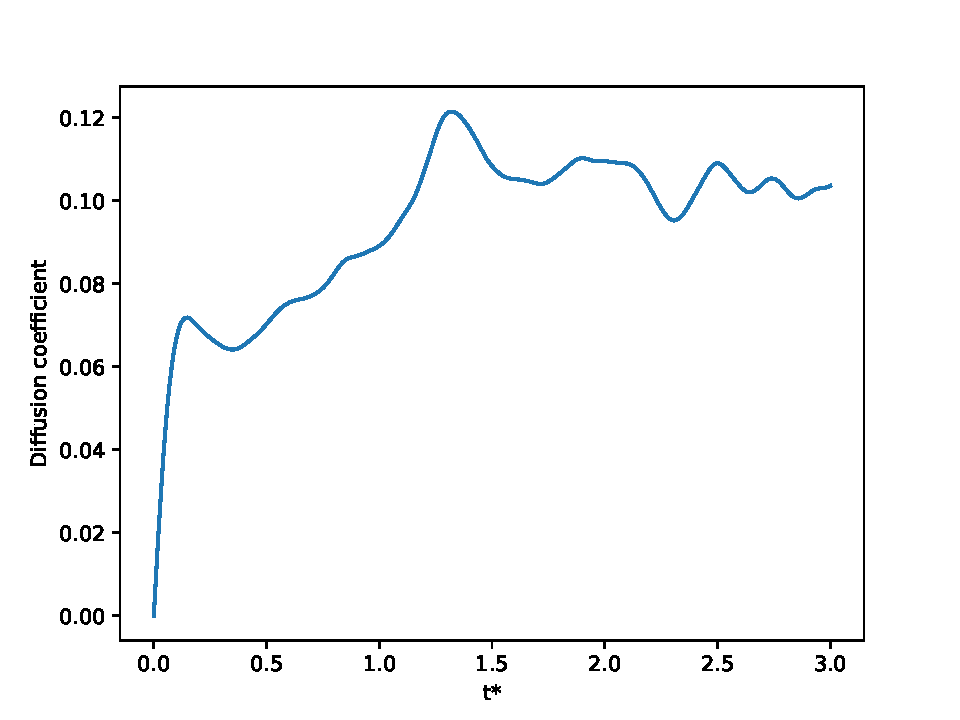
\includegraphics[scale=0.65]{../figures/4_b_v.pdf}
    \caption{Plot of diffusion coefficient for $t^* \in [0, 3]$.}
    \label{fig:diff}
\end{figure}

\subsection{Mean square displacement and diffusion coefficient} \label{4c}

We can also find the diffusion coefficient by looking at the slope mean square displacement over time. This is where we have to use our wallcount, which is the variable that counts how many time each atom has moved through any wall in any direction.

\begin{figure}[h!]
    \centering
    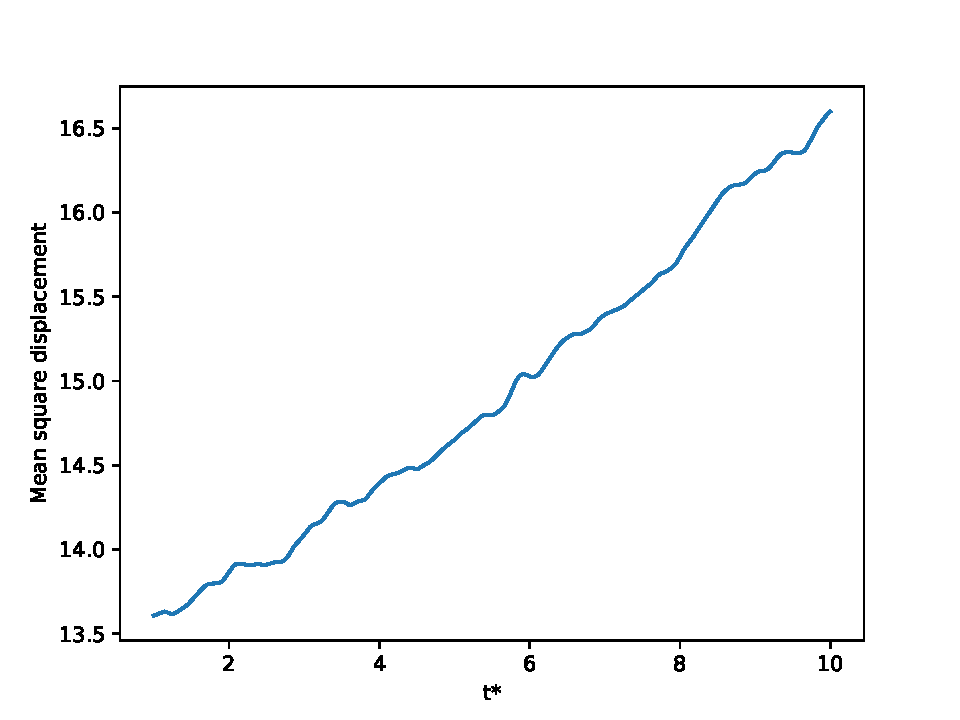
\includegraphics[scale=0.65]{../figures/4_c_ii.pdf}
    \caption{Mean square displacement for 864 atoms.}
    \label{msd}
\end{figure}

The slope of the linear part is approximately $0.3{r^*}^2/t^*$. This is $1.54 \cdot 10^{-4}$ cm$^2$s$^{-1}$, which is only a single order of magnitude bigger the value found by A. Rahman. 

\newpage

\subsection{Radial distribution function} \label{4d}

I did not vectorize the radial distribution function, so it takes quite a while. I added a progress bar instead. I ran a simulation with 1372 atoms for 10 $t^*$. It used 20 minutes to simulate and another 20 minutes to calculate the radial distribution. The results are shown below.

\begin{figure}[h!]
    \centering
    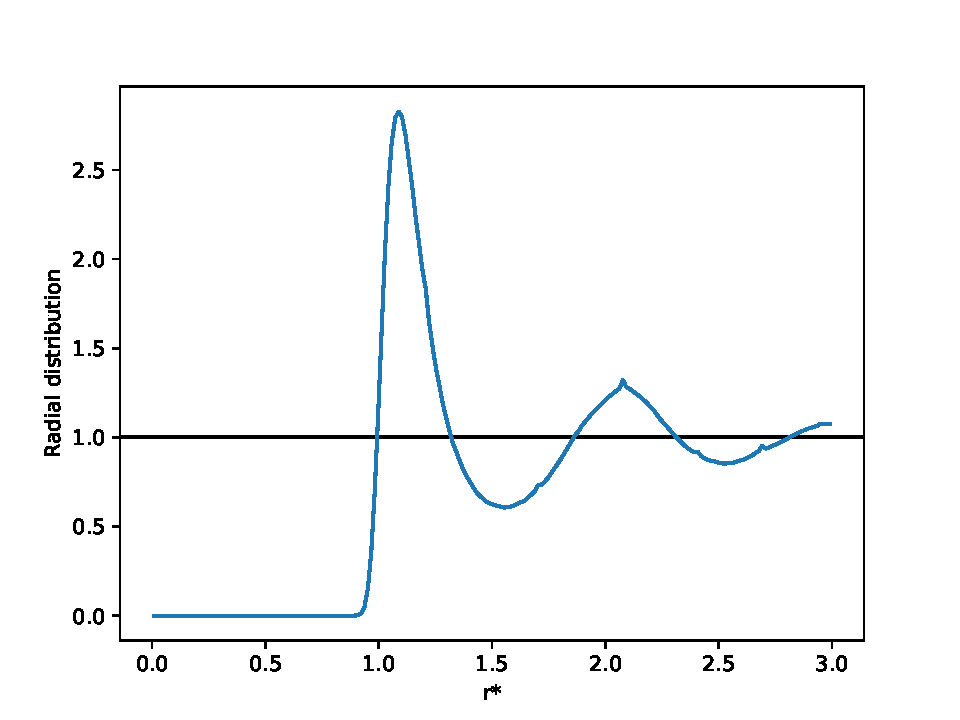
\includegraphics[scale=0.65]{../figures/4_d_i.pdf}
    \caption{Radial distribution for 1372 atoms.}
    \label{fig:rdf}
\end{figure}

A. Rahman used around 45 seconds per iteration when simulation 864 atoms. Note that he used a potential cutoff $r_c^* = 2.25 \sigma$, while my program uses $r_c^*=3 \sigma$, meaning that I have to calculate more per iteration. Yet, my program averages 12 iterations per second with $\Delta t = 0.01$ for 864 atoms. This is approximately 500 times as fast as A. Rahman. 

\end{document}